% 使用 XeLaTeX 编译两次；请在本文件所在目录执行。
\documentclass[UTF8,a4paper,11pt,fontset=fandol]{ctexart}
\usepackage[margin=2.3cm]{geometry}
\usepackage{amsmath,amssymb,booktabs,graphicx,tabularx}
\usepackage{float,placeins}
\usepackage[font=small,labelfont=bf]{caption}
\usepackage[hidelinks]{hyperref}
\usepackage{xurl}
\graphicspath{{figures/}}
\newcommand{\ket}[1]{\left|#1\right\rangle}
\newcommand{\bra}[1]{\left\langle#1\right|}
\newcommand{\Tr}{\operatorname{Tr}}
\newcommand{\Var}{\operatorname{Var}}
\newcommand{\dd}{\mathrm{d}}
\title{复数 RBM 的长时 projected p-tVMC 误差诊断\\
\large 基于全 Hilbert 空间求和的 Adam 基线研究}
\author{NeuralQuantumSolver 数值实验报告}
\date{2026年9月21日}
\begin{document}
\maketitle
\begin{abstract}
针对神经量子态在较长时间演化中出现投影误差增大和优化精度下降的现象，
本文研究一个十二格点、开放边界的 tilted-field Ising 淬火系统。
使用复数受限玻尔兹曼机（RBM）表示量子态，以 Adam 完成 projected p-tVMC 的逐步投影，
并通过全 Hilbert 空间求和开展三类诊断：冻结精确时间切片拟合、量子几何张量（QGT）谱分析、
以及 Schrödinger 演化方向的切空间投影残差。
在 $t=2$ 时，原始轨迹对精确对角化（ED）参考态的 infidelity 为 $0.2064$，
同一 RBM checkpoint 经独立的 ED 快照拟合后，所记录的最小 infidelity 为 $0.0250$。
QGT 在正时间采样点具有完整数值秩，但谱权重高度集中；末时刻有效秩为 $43.17$，
仅占 $636$ 个复参数的 $6.79\%$。末时刻归一化切空间残差为 $0.02857$。
这些结果表明，有限预算下的优化、逐步投影造成的轨迹偏离与局部切空间限制需要共同考虑。
它们尚不足以证明 RBM 的全局表达能力已经饱和，也不能将低有效秩直接解释为可删除参数的比例。
文中明确区分实验观测、推断和当前数据记录的数值限制。
\end{abstract}
\noindent\textbf{关键词：}神经量子态；RBM；projected tVMC；Adam；量子几何张量；切空间残差

\section{研究背景与问题}
长时 projected p-tVMC 的困难表现为：随着演化推进，每个时间步的投影优化不再达到早期的低误差，
最终 NQS 轨迹也逐渐偏离精确轨迹。增加隐藏单元或消除含时阶段的抽样噪声，并不自动保证问题消失。
因此需要把三个问题分别量化：第一，晚时刻精确态能否由给定大小的 RBM 较好地表示；第二，
参数数目是否对应足够多且数值条件良好的局部态变化方向；第三，当前态的精确演化方向有多少落在 RBM 切空间之外。

本文仅报告已完成的 Adam 实验。这里的“长时”指相对于本次 $t\in[0,2]$ 基线中误差显著增长的区间，
并不表示热力学极限或任意长时间的结论。A、B、C 是相互独立的观测：A 拟合冻结 ED 态，
B/C 则分析未经 A 再优化的原始 p-tVMC checkpoint。SR 结果不属于本文证据。

\section{物理模型与实验设置}
\subsection{Hamiltonian 与淬火协议}
采用代码中的 Pauli 矩阵约定，$\sigma_i^z$ 的本征值为 $\pm1$，取 $\hbar=1$：
\begin{equation}
H(J,h_x,h_z)=J\sum_{i=1}^{L-1}\sigma_i^z\sigma_{i+1}^z
-h_x\sum_{i=1}^{L}\sigma_i^x-h_z\sum_{i=1}^{L}\sigma_i^z.
\label{eq:hamiltonian}
\end{equation}
系统长度 $L=12$，采用开放边界。淬火前后参数分别为
\begin{equation}
(J_0,h_{x,0},h_{z,0})=(0,0.5,0),\qquad
(J_1,h_{x,1},h_{z,1})=(1,0.5,0.5).
\end{equation}
精确初态为 $H_0$ 的基态 $\ket{\psi_0}=\ket{+_x}^{\otimes12}$，基态能量为 $-6$。
淬火后以 $J_1=1$ 为能量单位。正号的 $J\sigma^z\sigma^z$ 项须与其他采用负号耦合约定的实现区别。

\subsection{RBM 参数化与归一化}
对构型 $x=(x_1,\ldots,x_L)$，$x_i=\pm1$，定义未归一化振幅
\begin{equation}
\widetilde\psi_\theta(x)=
\exp\!\left(\sum_i a_i x_i\right)
\prod_{j=1}^{M}2\cosh\!\left(b_j+\sum_i W_{ji}x_i\right),
\quad
\psi_\theta(x)=\frac{\widetilde\psi_\theta(x)}{\sqrt{\sum_y|\widetilde\psi_\theta(y)|^2}}.
\end{equation}
所有参数均为复数。复参数数目为
\begin{equation}
P=L+M+LM,
\qquad P_{4L}=636,\qquad P_{8L}=1260.
\end{equation}
这里 $P$ 是复参数数目，不是实坐标数目；相应实坐标数目为 $2P$。
随机重启使用代码的复数正态初始化，初始化尺度为 $0.01$。

\begin{table}[htbp]
\centering\small
\caption{Adam 基线设置。轨迹投影预算与 A 快照拟合预算不同。}
\label{tab:settings}
\begin{tabularx}{\linewidth}{lX}
\toprule
项目 & 设置 \\
\midrule
系统与精度 & $L=12$，$2^L=4096$ 个构型；PyTorch complex128；本轮配置记录为 CUDA \\
时间推进 & $\Delta t=0.05$，40 步，$t\in[0,2]$ \\
诊断时间 & $t=0,0.1,\ldots,2.0$，21 个 checkpoint \\
初态制备 & 4L 隐藏单元；Adam 100 步，学习率 $0.01$；seed=7 \\
初态抽样 & Metropolis 1000 条链；thermal sweeps=5；每链保留 1 个样本 \\
含时投影 & 每时间步重新创建 Adam；100 次更新；学习率 $0.01$ \\
A 拟合预算 & 每任务最多 1000 次 Adam 更新；停止阈值 $10^{-10}$ \\
A 学习率 & trajectory 与 4L 重启：$0.01$；8L 重启：$0.003$ \\
A 随机种子 & 4L、8L 各 5 个：1,2,3,4,5；trajectory 每时刻只拟合一次 \\
QGT 截断 & 相对阈值 $10^{-12}$；绝对阈值 0 \\
\bottomrule
\end{tabularx}
\end{table}
初态制备仍包含 MC 抽样；含时投影、ED 重叠和 A/B/C 均使用全空间求和。
因此这些阶段没有 MC 估计噪声，但初态训练误差、浮点误差与有限优化预算仍然存在。
原始 RBM 初态与 ED 初态的 infidelity 为 $1.0163\times10^{-7}$。

\section{数值方法与诊断定义}
\subsection{ED 参考与 projected p-tVMC}
设 $H_1=V\operatorname{diag}(E_n)V^\dagger$。ED 参考为
\begin{equation}
\ket{\psi_{\rm ED}(t)}=V\operatorname{diag}(e^{-iE_nt})V^\dagger\ket{\psi_0}.
\end{equation}
ED 时间切片直接在指定时刻计算，不通过逐步拟合生成。
同一谱分解给出 $U(\Delta t)=e^{-iH_1\Delta t}$，没有 Trotter 分解误差。
从当前 NQS 出发，单步冻结目标与优化问题为
\begin{align}
\ket{\phi_{n+1}}&=U(\Delta t)\ket{\psi_{\theta_n}},\\
\theta_{n+1}&\approx\arg\min_\theta
\left[1-|\langle\phi_{n+1}|\psi_\theta\rangle|^2\right].
\end{align}
每步从 $\theta_n$ 热启动，但 Adam 的动量状态重新初始化。RBM 参数而非 ED 态承接下一时间步。

必须区分局部与全局两个量：
\begin{align}
L_{\rm proj}^{\rm post}(t_{n+1})&=1-|\langle U(\Delta t)\psi_{\theta_n}|\psi_{\theta_{n+1}}\rangle|^2,
\label{eq:local}\\
L_{\rm ED}(t_n)&=1-|\langle\psi_{\rm ED}(t_n)|\psi_{\theta_n}\rangle|^2.
\label{eq:global}
\end{align}
式\eqref{eq:local}从已有近似态出发，式\eqref{eq:global}从精确初态出发。
局部误差不能直接相加得到全局 infidelity；相位、误差方向及后续幺正传播均会影响累积。

\paragraph{原始 CSV 的记录约定。}
当前 Adam 轨迹代码在第100次更新之前计算并保留变量 \texttt{projection\_loss}，
而 \texttt{step\_fidelity} 在该次更新之后重新评估。
因此已有图中的局部曲线严格对应最后一次更新前的 loss；真正更新后的量是
$L_{\rm proj}^{\rm post}=1-\texttt{step\_fidelity}$。
本文保留既有图片并明确这一差别，不将二者误认为逐位一致。

\subsection{A：冻结精确时间切片拟合}
对每个 $t_k$，以固定的 $\ket{\psi_{\rm ED}(t_k)}$ 为目标，优化
\begin{equation}
\mathcal L_A(\theta;t_k)=1-|\langle\psi_{\rm ED}(t_k)|\psi_\theta\rangle|^2.
\end{equation}
比较三类初始化：原始4L轨迹 checkpoint、随机初始化的4L RBM、随机初始化的8L RBM。
后两类各使用5个种子；各时间点独立拟合，不把上一个快照的拟合结果传给下一个。
trajectory 的 seed 字段不表示另有5条动力学轨迹。

若 $k$ 表示实际被评估的优化迭代，记录
\begin{equation}
\mathcal L_{\rm best}^{(s)}(t)=\min_{k\in\mathcal K}\mathcal L_A(\theta_k^{(s)};t),
\quad
\mathcal L_{\min}(t)=\min_s\mathcal L_{\rm best}^{(s)}(t),
\quad
\mathcal L_{\rm med}(t)=\operatorname{median}_s\mathcal L_{\rm best}^{(s)}(t).
\end{equation}
中位数反映典型重启表现，最小值反映本轮搜索找到的最好结果；二者都不是全局最优性的证明。
真实表示误差下界满足
\begin{equation}
\inf_\theta\mathcal L_A(\theta;t)\leq \mathcal L_{\min}(t).
\end{equation}
因此非零拟合误差只能给出已达到误差水平，不能证明此精确态一定超出 RBM 的表示集合。
总计执行 $21(1+5+5)=231$ 个拟合任务。

\subsection{B：QGT 谱与有效秩}
定义对数导数与 Born 权重
\begin{equation}
O_i(x)=\partial_{\theta_i}\log\widetilde\psi_\theta(x),\qquad
p(x)=|\psi_\theta(x)|^2,\qquad \langle A\rangle_p=\sum_xp(x)A(x).
\end{equation}
复解析 RBM 的 QGT 为
\begin{equation}
S_{ij}=\langle O_i^*O_j\rangle_p-\langle O_i^*\rangle_p\langle O_j\rangle_p.
\end{equation}
设本征值为 $\lambda_i$，截断阈值 $\tau=10^{-12}\lambda_{\max}$，则
\begin{align}
r_{\rm num}&=\#\{i:\lambda_i>\tau\}, &
r_{\rm eff}&=\frac{(\sum_i\lambda_i)^2}{\sum_i\lambda_i^2},\\
\kappa_{\rm ret}&=\frac{\max_{\lambda_i>\tau}\lambda_i}{\min_{\lambda_i>\tau}\lambda_i}, &
f_{\rm eff}&=r_{\rm eff}/P.
\end{align}
代码保留原始谱，计算有效秩时将舍入造成的微小负值截为0。
$r_{\rm eff}$ 是谱参与率，不是非零本征值的数目；它也随参数坐标的缩放而改变。
因此它描述当前参数化下的谱集中程度，不等于“有效使用了多少个可独立删除的参数”。

\subsection{C：投影 Hilbert 空间中的切空间残差}
对归一化态，移除平行于态本身的规范分量后，定义
\begin{equation}
J_{xi}=\psi_\theta(x)\left[O_i(x)-\langle O_i\rangle_p\right],
\quad q=(H_1-\langle H_1\rangle)\ket{\psi_\theta}.
\end{equation}
这里 $J$ 为投影后的 Hilbert 空间 Jacobian，$S=J^\dagger J$。
令 $F=J^\dagger q$，$\Var(H_1)=q^\dagger q$，并按与 B 一致的谱阈值定义 $S_\tau^+$。
当方差非零时，
\begin{equation}
R_{\rm tan}=1-\frac{F^\dagger S_\tau^+F}{\Var(H_1)}
=\frac{\min_v\|Jv+iq\|^2}{\|q\|^2}.
\label{eq:tangent}
\end{equation}
右侧最小化仅使用与截断伪逆相同的保留切空间。
使用 $J=U\Sigma V^\dagger$ 的显式 SVD，保留 $\sigma_i^2>\tau$，得到独立的最小二乘检查。
代码对因消减误差而略小于0的残差作非负截断，方差近零时则将归一化量标为未定义。

$R_{\rm tan}$ 是\textbf{平方范数比例}，不是 ED infidelity。
在无截断理想切空间、无穷小时间步和精确局部投影的假设下，有
\begin{equation}
L_{\rm proj}^{\rm ideal}(\Delta t)
=\Delta t^2\Var(H_1)R_{\rm tan}+o(\Delta t^2).
\label{eq:local-asymptotic}
\end{equation}
这解释了切空间残差与局部投影困难的联系，但不能据此精确预测有限步长、有限优化预算的结果。

\section{结果}
\subsection{原始 trajectory 的局部与全局误差}
图\ref{fig:rollout}中，全局 ED infidelity 从 $1.0163\times10^{-7}$ 增长到
$t=0.5$ 的 $0.008435$、$t=1.5$ 的 $0.130861$ 和 $t=2$ 的 $0.206419$。
末步 CSV 的局部 loss 为 $0.00153868$；由末步更新后的保真度得到
$L_{\rm proj}^{\rm post}(2)=0.001533924$。
局部约千分之一的误差与累计约两成的 infidelity 可以同时存在，
因为每一步都沿已偏离 ED 的近似态继续推进。
\begin{figure}[htbp]
\centering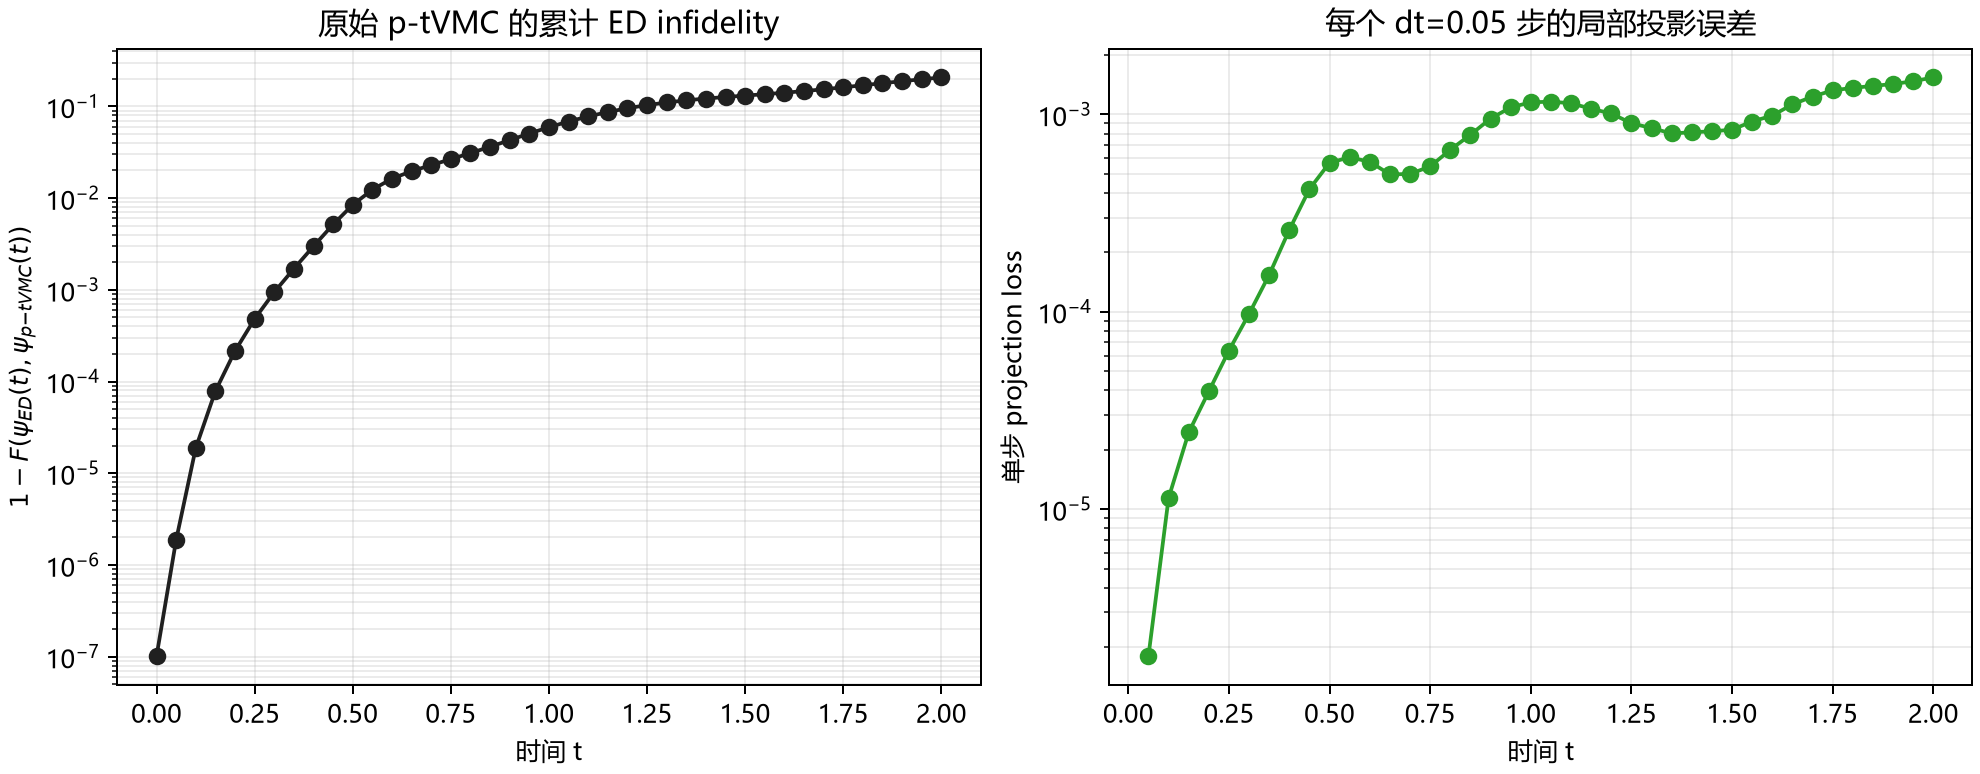
\includegraphics[width=\linewidth]{rollout_quality.png}
\caption{Adam 原始轨迹：左为 $L_{\rm ED}$；右为原 CSV 的最后一次内部更新前
\texttt{projection\_loss}。右图时间标记为该步终点。精确更新后误差应使用
$1-\texttt{step\_fidelity}$。}
\label{fig:rollout}
\end{figure}

\subsection{A：轨迹之外仍存在更低误差的 RBM}
\begin{table}[htbp]
\centering\small
\caption{A 的代表性时间点。随机重启列分别报告5个种子的最小值和中位数；所有误差均对 ED 态计算。}\label{tab:a}
\resizebox{\linewidth}{!}{%
\begin{tabular}{ccccccc}
\toprule
$t$ & 轨迹原始 & 轨迹再拟合 & 4L 最小 & 4L 中位 & 8L 最小 & 8L 中位 \\
\midrule
0.0 & $1.016\times10^{-7}$ & $9.991\times10^{-11}$ & $8.599\times10^{-11}$ & $9.479\times10^{-11}$ & $5.305\times10^{-11}$ & $9.270\times10^{-11}$ \\
0.5 & $8.435\times10^{-3}$ & $2.760\times10^{-5}$ & $4.945\times10^{-5}$ & $5.922\times10^{-5}$ & $2.068\times10^{-4}$ & $2.130\times10^{-4}$ \\
1.0 & $5.919\times10^{-2}$ & $3.249\times10^{-3}$ & $3.500\times10^{-3}$ & $3.833\times10^{-3}$ & $2.742\times10^{-3}$ & $2.940\times10^{-3}$ \\
1.5 & $1.309\times10^{-1}$ & $1.692\times10^{-2}$ & $1.574\times10^{-2}$ & $1.647\times10^{-2}$ & $1.064\times10^{-2}$ & $1.195\times10^{-2}$ \\
2.0 & $2.064\times10^{-1}$ & $2.500\times10^{-2}$ & $2.911\times10^{-2}$ & $3.008\times10^{-2}$ & $2.824\times10^{-2}$ & $3.128\times10^{-2}$ \\
\bottomrule
\end{tabular}}
\end{table}

表\ref{tab:a}与图\ref{fig:a}显示，独立快照拟合可明显改善同一尺寸 RBM 的 ED 重叠。
例如 $t=2$ 时由 $0.206419$ 降至本轮记录的 $0.0249995$，相差约8.26倍。
这表明原始轨迹并未在每个时间点都达到该 RBM 已能达到的 ED 拟合精度。
但重新拟合使用了精确终态信息与更大的预算，它不是实际未知 ED 态时可直接使用的时间推进方案。
这一改善也不能定量分解为某个确定比例的“纯优化误差”。

在 $t=1.5$，4L 随机重启的最佳值为 $0.01574$，8L 为 $0.01064$；
在 $t=2$，两者分别约为 $0.02911$ 和 $0.02824$。
扩大网络的优势依赖时间点，且8L学习率也从 $0.01$ 改为 $0.003$，故本轮不是仅改变容量的严格消融。
在 $t=1$ 的8L重启中，一个 seed 的最佳 loss 约 $0.09187$，而其余多个 seed 约为 $0.003$，
说明仅报告跨 seed 最小值会掩盖优化失败或较差局部解。

231个拟合中，只有 $t=0$ 的11个任务达到 $10^{-10}$ 停止阈值。
其余220个任务达到1000步预算，因此本轮没有充分证据称其均已达到收敛平台。
\begin{figure}[htbp]
\centering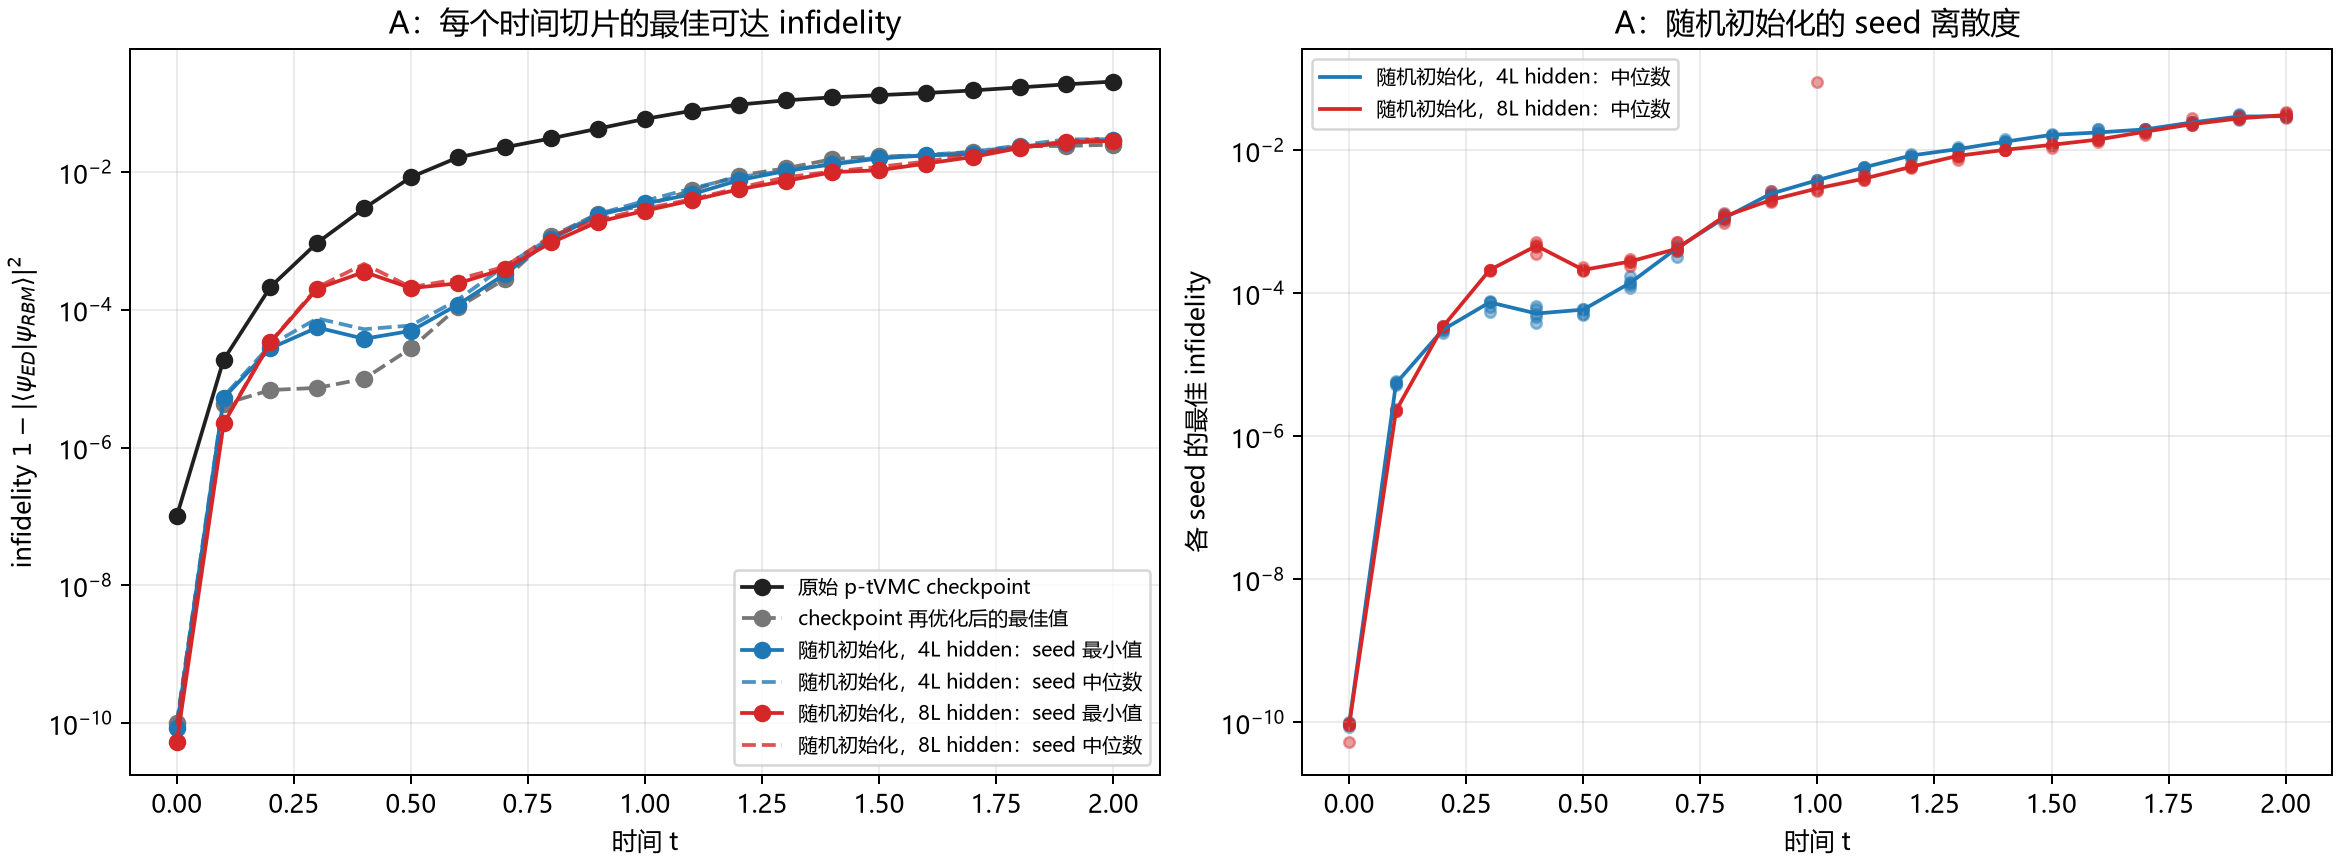
\includegraphics[width=\linewidth]{a_snapshot_infidelity.png}
\caption{A：所有纵坐标均为对冻结 ED 态的 infidelity。左图区分原始 trajectory、
checkpoint 再优化和两种随机重启；右图显示5个种子的散点与中位数。
既有图片标题中的“最佳可达”仅指本轮有限预算内实际评估到的最小值。}
\label{fig:a}
\end{figure}

\subsection{B：满数值秩与低有效秩并存}
\begin{table}[htbp]
\centering\small
\caption{B/C 的代表性数值，均在原始4L轨迹上测量。初态残差为代码截断后的值。}\label{tab:bc}
\resizebox{\linewidth}{!}{%
\begin{tabular}{cccccc}
\toprule
$t$ & $r_{\rm num}$ & $r_{\rm eff}$ & $r_{\rm eff}/P$ & $\kappa_{\rm ret}$ & $R_{\rm tan}$ \\
\midrule
0.0 & 613 & 13.14 & 2.07\% & $9.771\times10^{11}$ & $0.000\times10^{0}$ \\
0.5 & 636 & 56.07 & 8.82\% & $6.670\times10^{6}$ & $4.795\times10^{-3}$ \\
1.0 & 636 & 54.97 & 8.64\% & $4.468\times10^{8}$ & $1.805\times10^{-2}$ \\
1.5 & 636 & 50.03 & 7.87\% & $5.263\times10^{7}$ & $1.281\times10^{-2}$ \\
2.0 & 636 & 43.17 & 6.79\% & $1.523\times10^{7}$ & $2.857\times10^{-2}$ \\
\bottomrule
\end{tabular}}
\end{table}

在全部正时间诊断点，$r_{\rm num}=636$，并未观察到相对于当前截断阈值的严格降秩。
有效秩在早期先增大，随后出现波动并在后期下降；$t=0.5$ 为56.07，$t=2$ 为43.17。
末时刻 $f_{\rm eff}=0.06787$，表明谱权重集中在少数较强方向。
保留条件数在 $t=0$ 约为 $9.77\times10^{11}$，$t=2$ 约为 $1.52\times10^7$，
中间时刻并非单调增长。因此不能把“晚时刻误差增长”直接等同于“条件数持续恶化”。
图\ref{fig:b}与图\ref{fig:spectrum}展示了标量指标与谱的区别。
\begin{figure}[htbp]
\centering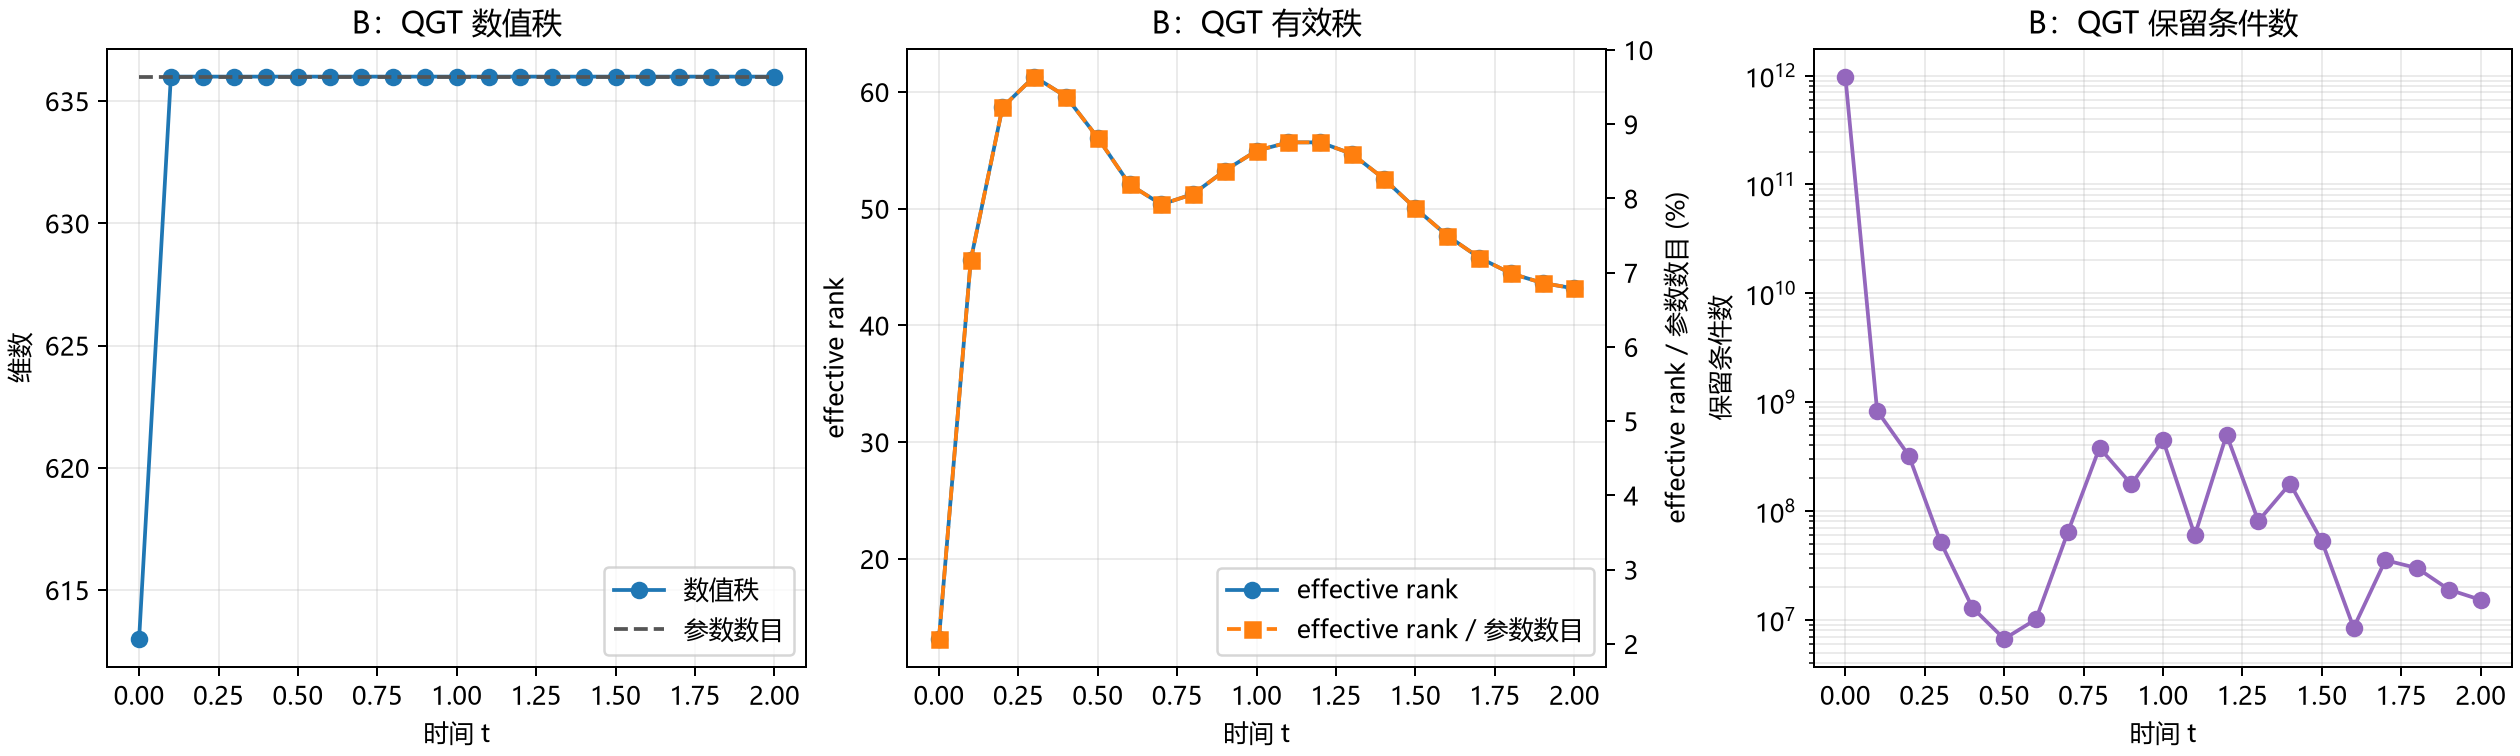
\includegraphics[width=\linewidth]{b_qgt_scalars.png}
\caption{B：原始4L trajectory 的 QGT 数值秩、有效秩及比例、保留条件数。
中间面板比例由右轴按百分数读取。B 未使用 A 再优化后的模型，也未给出8L轨迹的秩扫描。}
\label{fig:b}
\end{figure}
\begin{figure}[htbp]
\centering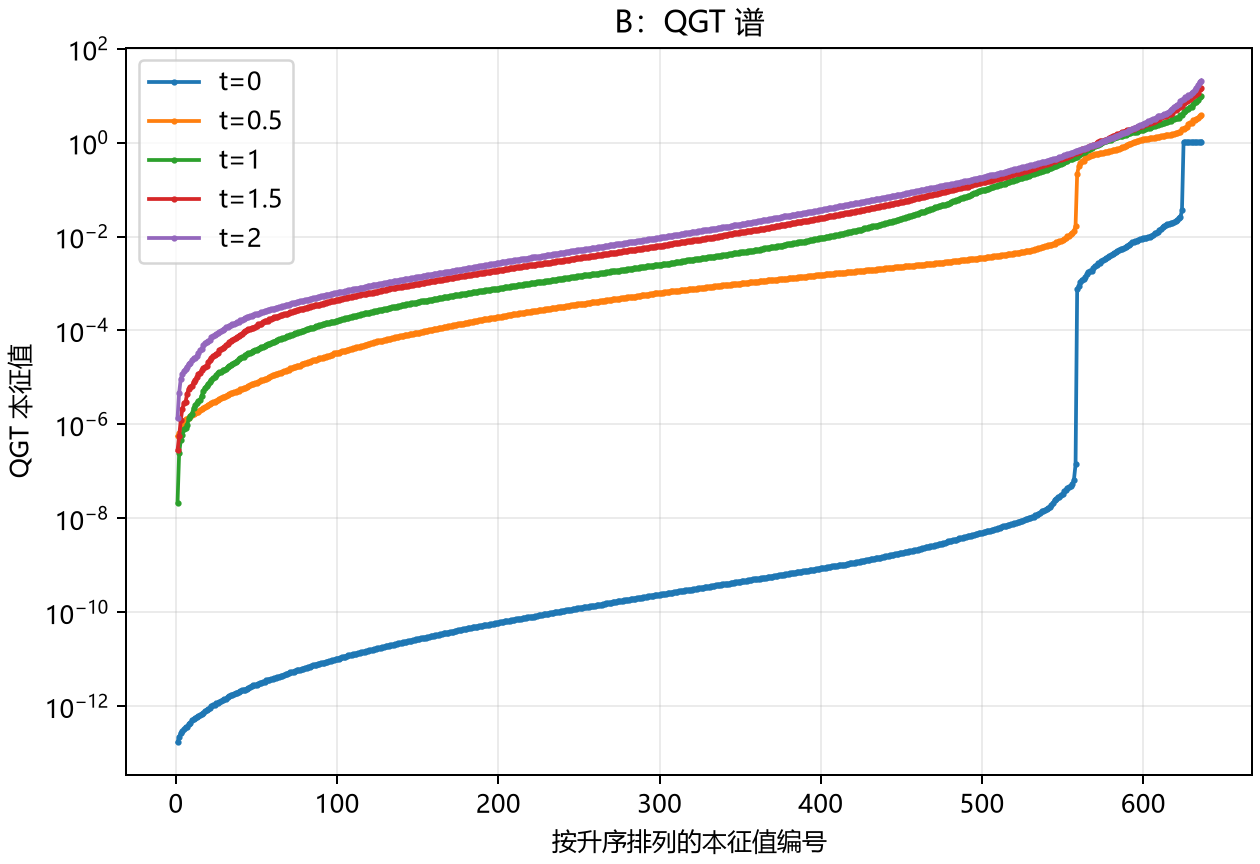
\includegraphics[width=0.78\linewidth]{b_qgt_spectra.png}
\caption{若干时刻原始4L trajectory 的 QGT 本征值，按升序排列，纵轴采用对数刻度。
跨越多个数量级的谱与满数值秩并不矛盾。}
\label{fig:spectrum}
\end{figure}

\subsection{C：局部切空间限制随时间发生变化}
$R_{\rm tan}$ 在 $t=0.5,1.0,1.5,2.0$ 分别约为
$0.004795,0.01805,0.01281,0.02857$。
它整体较初期增大但不单调，也没有在 $t=1.5$ 出现由本数据支持的突变。
末时刻有约 $2.86\%$ 的中心化 Schrödinger 方向平方范数落在保留切空间之外，
对应范数比例 $\sqrt{R_{\rm tan}}\simeq16.9\%$。
这里计算的是当前 RBM 状态的演化方向，不是直接计算精确 ED 态的切空间距离。

两种残差计算在正时间点的最大绝对差约为 $2.20\times10^{-10}$，见图\ref{fig:c}。
$t=0$ 的 QGT 公式经非负截断后为0，而显式最小二乘给出 $9.06\times10^{-9}$；
这一差异与近奇异 QGT 及两个相近大数相减的数值敏感性相容，不能据此断言残差严格为零。
对初态及极小残差的结论仍需要截断阈值敏感性检验。
\begin{figure}[htbp]
\centering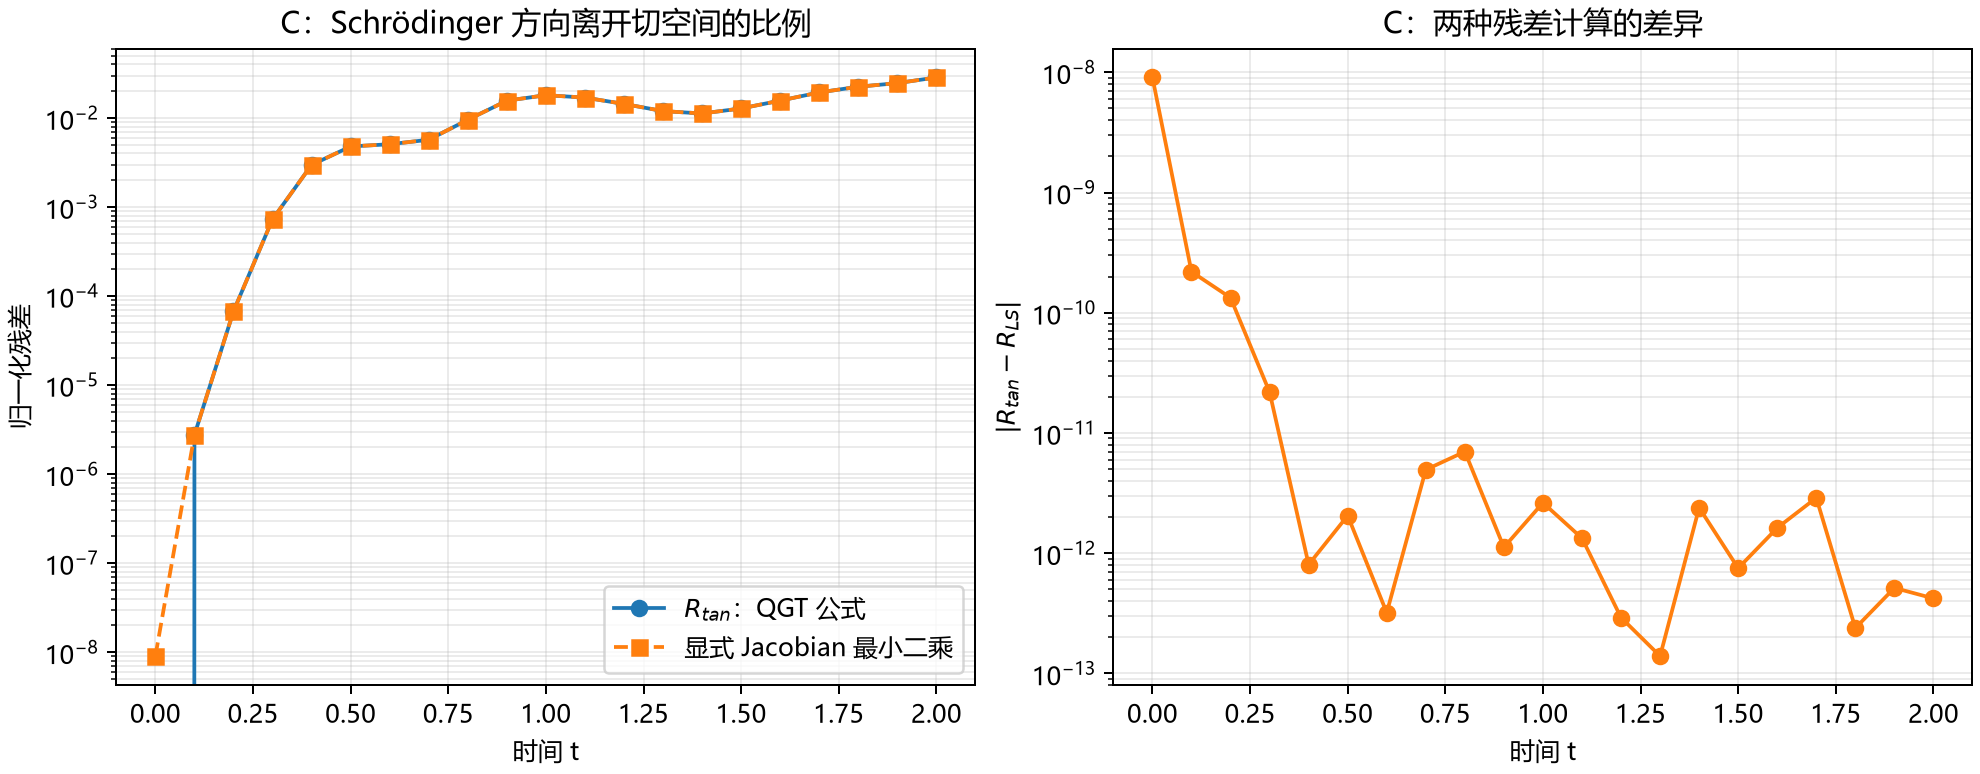
\includegraphics[width=\linewidth]{c_tangent_residual.png}
\caption{C：左为 QGT 公式和显式 Jacobian 最小二乘残差，右为两者的绝对差。
零值不能在对数纵轴上正常显示，故左图 $t=0$ 的 QGT 结果不可按曲线外推解读。
右图保留初态约 $10^{-8}$ 的交叉验证差异。}
\label{fig:c}
\end{figure}
\FloatBarrier

\section{讨论：可以支持与尚不能支持的结论}
\paragraph{表示能力与优化。}
A 表明同一4L网络能够达到比原始 trajectory 更低的 ED infidelity，
因此把全部长时误差解释为容量不足是不充分的。
然而残余约 $0.025$ 是有限优化的上界结果；没有全局优化证明或预算收敛研究，
不能把它当作该网络的不可消除表示误差。
warm-start 在部分时间点仍有优势，但1000步后的随机重启已达到相近量级，
因而“轨迹携带信息，所以必然远优于随机初始化”也不是这轮数据的普遍结论。

\paragraph{有效秩与参数效率。}
低有效秩说明当前坐标下 QGT 谱不均匀，而正时间满数值秩说明许多小权重方向仍独立存在。
不能据此说剩余约90\%参数完全无用。
此外，本轮 B 只沿4L轨迹测量，尚未比较增加网络宽度后的 QGT；
关于“参数增加而有效秩饱和”的原始问题仍未得到直接检验。

\paragraph{局部切空间与长时偏离。}
C 提供了局部几何限制的直接量化，并与原始轨迹的局部投影困难相容。
但局部切空间残差、有限 $\Delta t$ 下的非线性变分投影、Adam 优化不足及全局误差传播不是同一个量。
快照拟合存在更好解，也不保证从前一时刻沿小步优化一定可到达它。

\paragraph{后续对照。}
在保留 Adam 结果的前提下，SR 应分别用于含时投影与 A 的冻结态拟合；
B/C 则继续用相同定义分析新轨迹。
比较时应同时记录迭代次数、实际时间、正则化与谱截断，尽量复用同一 $t=0$ checkpoint，
并进行步长和迭代预算敏感性研究。只有这些对照完成后，才能判断几何预条件是否实际改善长时精度。

\section{结论}
本次十二格点 Adam 全求和实验同时观测到：显著的全局轨迹偏离、
独立 ED 快照拟合带来的明显改善、满数值秩但高度集中的 QGT 谱，以及后期增大的切空间残差。
证据支持将优化可达性、局部几何与误差传播结合分析，而不是将长时失效归结为单一因素。
当前数据尚不能确定网络的最优表示误差下界，不能证明随网络宽度增长的有效秩饱和，
也不能预先保证 SR 必然解决问题。

\appendix
\section{数据、代码与记录限制}
本报告基于仓库中的本地实验数据，不作为外部文献综述。图像来自已生成的 Adam 图，
以副本固定在文稿目录；数值表由原始 CSV 自动生成。输入文件散列与数据数量见
\path{data_manifest.json}，可用于确认后续是否引用了同一轮数据。

\begin{table}[htbp]
\centering\small
\caption{报告量与数据字段的映射。所有结果路径相对于仓库根目录。}
\begin{tabularx}{\linewidth}{lX}
\toprule
量 & 来源与解释 \\
\midrule
原始轨迹 & \path{benchmark_results/projected_ptvmc_trajectory/trajectory.csv}，41行 \\
$L_{\rm ED}$ & 上述文件的 $1-\texttt{ed\_fidelity}$ \\
$L_{\rm proj}^{\rm post}$ & 上述文件的 $1-\texttt{step\_fidelity}$；初态不定义 \\
A 的结果 & 诊断目录 \path{results.csv} 中带 \texttt{family} 的231行 \\
B/C 的结果 & 同一 CSV 中 \texttt{family} 为空的21行 \\
完整 QGT 谱 & 同目录 \path{summary.json} 的 \texttt{qgt\_spectra} \\
配置 & 同目录 \path{config.json} 与轨迹目录 \path{run_config.json} \\
\bottomrule
\end{tabularx}
\end{table}
这里诊断目录为
\begin{quote}\small\path{benchmark_results/diagnostics/late_time_snapshot_adam_1000_seed5}\end{quote}
主要实现位于 \path{examples/time_evolution/projected_time_evolution.py}、
\path{examples/diagnostics/exact_snapshot_diagnostics.py} 以及
\path{src/neural_quantum_solver/diagnostics/}。

\paragraph{A 的 checkpoint 与 loss 对齐问题。}
当前 Adam 拟合循环先计算 $\mathcal L(\theta_k)$，随后执行更新得到 $\theta_{k+1}$，
再根据更新前的 loss 判断是否保存参数。
因此 \texttt{best\_loss} 是实际评估过的数值，但配套 \texttt{best\_state\_dict} 可能来自下一次参数状态；
\texttt{final\_loss} 也是最后一次更新前的值。
这不使 CSV 中观测到的 infidelity 无效，却意味着直接重载 \texttt{checkpoints.pt}
未必能复现对应的 \texttt{best\_loss}。
正式做 checkpoint 级比较前，需要重算其 loss 并修正后续实验的记录顺序。
本文未修改或覆盖既有数据，也未声称已对所有保存的最佳模型进行了再验证。

\paragraph{统计与复现范围。}
5个重启种子的离散度不等于跨独立物理轨迹的统计误差条；
同一 seed 在不同时间点重复使用，亦不构成时间之间的独立抽样。
当前结果仅覆盖一种系统大小、一条初始轨迹及有限超参数设置。
记录 seed 和配置有助于复现，但不能保证不同硬件与后端的逐位一致。
\end{document}
